% !TeX spellcheck = cs_CZ
%{\tikzset{external/prefix={tikz/FYZI/}}
% \tikzset{external/figure name/.add={ch24_}{}}
%=========================== Kapitola: Přechodové jevy ============================================
\setchaptertoc
\chapter{Přechodové jevy}\label{fyz:IchapXXIV}

  \section{Energie oscilátoru}\label{fyz:IchapXXIVsecI}
  \section{Tlumené kmity}\label{fyz:IchapXXIVsecII}
  \section{Přechodové jevy v elektrických obvodech}\label{fyz:IchapXXVIVsecIII}
  \section{Příklady a cvičení}\label{fyz:IchapXXIVsecIV}

    \begin{figure}[ht!] %\ref{fyz:fig0300}
      \centering
      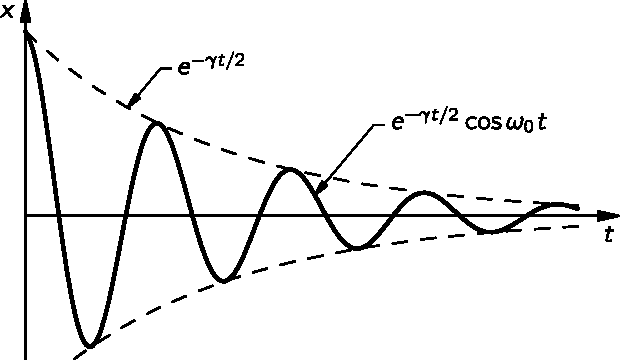
\includegraphics[width=0.7\linewidth]{fyz_fig0300.pdf}
      \caption{Tlumené kosinové oscilace 
               (\cite[s.~326]{Feynman01})}
      \label{fyz:fig0300}
    \end{figure}

    \begin{figure}[ht!] %\ref{fyz:fig0301}
      \centering
      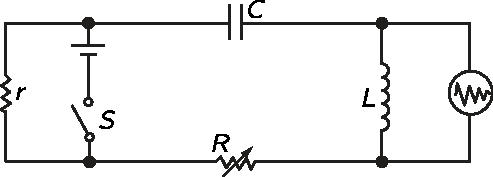
\includegraphics[width=0.7\linewidth]{fyz_fig0301.pdf}
      \caption{Demonstrace přechodových jevů na elektrickém obvodu 
               (\cite[s.~328]{Feynman01})}
      \label{fyz:fig0301}
    \end{figure}
    

    \begin{figure}[ht!]      %\ref{fyz:fig0302}
      \centering
      \subcaptionbox{\label{fyz:fig0302a}}{\luafigure[0.45]{fyz_fig0302a.pdf}}
      \subcaptionbox{\label{fyz:fig0302b}}{\luafigure[0.45]{fyz_fig0302b.pdf}}         \\
      \subcaptionbox{\label{fyz:fig0302c}}{\luafigure[0.45]{fyz_fig0302a.pdf}}
      \subcaptionbox{\label{fyz:fig0302d}}{\luafigure[0.45]{fyz_fig0302b.pdf}}         
      \caption{Příklady tlumených oscilací vyfotografovaných z obrazovky osciloskopu
               \cite[s.~329]{Feynman01}}
      \label{fyz:fig0302}
    \end{figure}

    \todo[inline]{Kapitola fey1ch24 je zcela prázdná, pouze obrázky}  
%} %tikzset
%---------------------------------------------------------------------------------------------------